\documentclass{utue} %uumi.cls required for Uni Ulm corporate design
\usepackage{listings}
\usepackage{caption}
\usepackage{geometry}
\usepackage{url}
\usepackage{amssymb}
\usepackage{mathrsfs}
\usepackage{tikz}
\usepackage{subcaption}

\lstset{
basicstyle=\rmfamily,
columns=fullflexible,
frame=tb,
framexleftmargin=20pt,
captionpos=t,
breaklines=true,
mathescape,
numbers=left,
numberstyle=\small,
numbersep=5pt,
xleftmargin=20pt,
tabsize=3,
escapeinside={\{}{\}},
keywords={Input, Output, if, else, then, return, for, all, do}
}
\DeclareCaptionFormat{listing}{\hrule#1#2#3}
\captionsetup[lstlisting]{format=listing,singlelinecheck=false, margin=0pt,labelsep=space,labelfont=bf}
\renewcommand*\thelstnumber{\arabic{lstnumber}:}

% Values for title generation
\title{Dual tree traversal for nearest neighbour search}
\author{Fabian Fritz}
\date{\today}

% Subtitle is optional. It represents what kind of work you did.
\subtitle{Praktikum Computergrafik SoSe2016}

\begin{document}

% You can place a teaser as follows. (Otherwise, just uncomment the following part)
\teaser{
    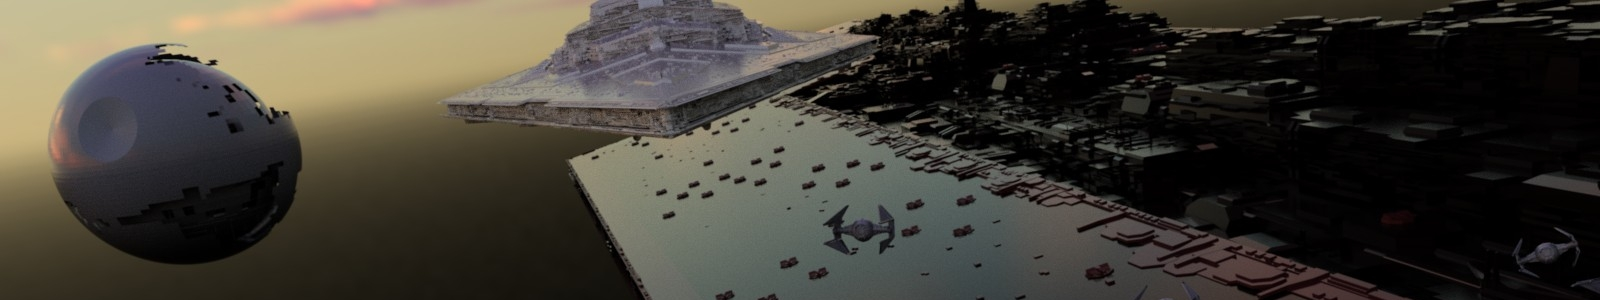
\includegraphics[width=\textwidth]{images/teaser.jpg}
    \caption{You can place a teaser here.}
    \label{fig:teaser}
}     

% Creates title of document and additional title page.
\maketitle

\section*{Abstract}

Give an overview over your project here. Give a glimpse insight in the problem and write why it is important to be solved. Write what you did to make your implementation better than the state of the art implementations.


\section{Introduction}

Aligning two sets of points in multiple dimensions (known as point set registration or point matching) is an important step if one is interested in comparing two point clouds.
These points might originate from an accurate 3d model of an object, a 3d scan or from other tools to acquire multidimensional data. Even if the same method was used for both sets, the number of points and their exact positions might differ. Also, in case the two sets actually have the same number of points, one cannot assume the points appear in the same order. Let $\mathbf{Q},\mathbf{P}$ be two point sets, $\mathbf{q} \in \mathbf{Q}, \mathbf{p} \in \mathbf{P}$ be points in the respective set. To align the two sets, it is necessary then to find a transformation$$
\min \sum_{i,j}^{|P|,|Q|} |\mathbf{p_i}-\mathcal{T}(\mathbf{q_j})|
$$
where $\mathcal{T}(\mathbf{Q}) = s\mathbf{R}\mathbf{Q} + \mathbf{t}$ is a rigid transformation of set $\mathbf{Q}$ with $s$ being the scaling factor, $\mathbf{R}$ being a rotation matrix and $\mathbf{t}$ being a translation vector. This is also known as a Procrustes transformation.

The iterative-closest-point (ICP) algorithm solves both problems: finding the best corespondence between the sets of points and aligning the point clouds according to this. To do this, it is necessary first to find the nearest neighbor for each point. Then, the sets of points can be aligned by minimizing the total distance between the points. These two steps are repeated until either the point clouds are perfectly aligned or the total distance is below some specified threshold.

While the second step, minimizing the distances between points, can be trivially implemented, e. g. by using the least squares method, there are multiple ways of implementing and optimizing the nearest neighbor search (NNS). One way of improving the performance of an NNS is by using dedicated data structures, such as trees, for either one or both sets of points. The method of using treelike structures for both sets is known as dual-tree traversal.

There is a large variety of trees one can use in conjunction with the dual tree traversal algorithm, and their influence on the performance has already been studied comprehensively. However, little was done to investigate how to run this algorithm in parallel. In particular, the possibility of utilizing the graphics processing unit(GPU) as a means of computation for this search hasn't been explored thoroughly.

With this work we want to advance Curtis' work \cite{improving} towards a parallel implementation of this general approach. By comparing the performance of a brute-force approach and search on a single kdtree and search on two R-trees, both in the sequential as well as the parallel way, we show 
\section{Related Work} 

The ICP already was described in 1992. Since then, many optimizations have been proposed.

\section{Description of the Solution}
\begin{figure}
	\begin{subfigure}{.24\textwidth}
		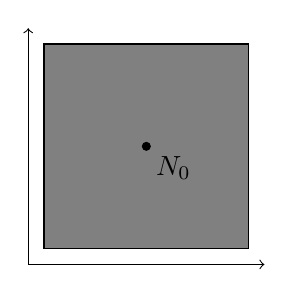
\begin{tikzpicture}
		\draw[->] (0,0) -- (0,3);
		\draw[->] (0,0) -- (3,0);
		\draw[fill=gray] (0.2,0.2) rectangle (2.8,2.8) node[pos=.5,circle,draw=black,fill=black,inner sep=1pt] (nodeanchor) {};
		\node[below right] at (nodeanchor) {$N_0$};
		\end{tikzpicture}
	\end{subfigure}
	\begin{subfigure}{.24\textwidth}
	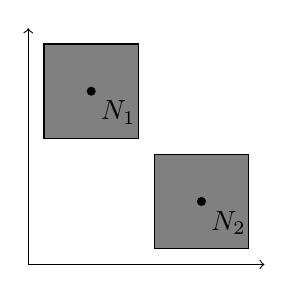
\begin{tikzpicture}
		\draw[->] (0,0) -- (0,3);
		\draw[->] (0,0) -- (3,0);
		\draw[fill=gray] (0.2,1.6) rectangle (1.4,2.8) node[pos=.5,circle,draw=black,fill=black,inner sep=1pt] (nodeanchor) {};
		\draw[fill=gray] (1.6,0.2) rectangle (2.8,1.4) node[pos=.5,circle,draw=black,fill=black,inner sep=1pt] (nodeanchor2) {};
		\node[below right] at (nodeanchor) {$N_1$};
		\node[below right] at (nodeanchor2) {$N_2$};
	\end{tikzpicture}
	\end{subfigure}
	\caption{R-tree at root level and the level below.}
\end{figure}
\begin{lstlisting}[caption={Simple \texttt{BaseCase()} for nearest neighbor search.}]
Input: query point $p_q$, reference point $p_r$, candidate point $N[p_q]$, candidate distance $D[p_q]$
Output: distance $d(p_q,p_r)$
if $d(p_q,p_r) < D[p_q]$ then
	$N[p_q] \leftarrow p_r$
	$D[p_q] \leftarrow d(p_q, p_r)$
\end{lstlisting}
\begin{lstlisting}[caption={Simple \texttt{Score()} for nearest neighbor search}]
Input: query node $\mathscr{N}_q$, reference node $\mathscr{N}_r$
Output: a score for the node combination $(\mathscr{N}_q, \mathscr{N}_r)$ or $\infty$ if it should be pruned
if $d_{min}(\mathscr{N}_q, \mathscr{N}_r) > B_{df}(\mathscr{N}_q)$ then
	return $\infty$
return $d_{min}(\mathscr{N}_q, \mathscr{N}_r)$
\end{lstlisting}

\begin{lstlisting}[caption={\texttt{DualTraversal}($\mathscr{N}_q,\mathscr{N}_r$)}]
Input: query node $\mathscr{N}_q$, reference node $\mathscr{N}_r$
{\{Calculate bound and prune if possible.\}}
$\{\mathscr{D}^p(\mathscr{N}_q)$ represents the set of descendant points of the query node $\mathscr{N}_q$}
$b\leftarrow \max_{p \in \mathscr{D}^p(\mathscr{N}_q)}D_{p_q}$
if $d_{min}(\mathscr{N}_q, \mathscr{N}_r) > b$ then
	return
if $\mathscr{N}_q$ and $\mathscr{N}_r$ are both leaves then
	BaseCase($p_q$, $p_r$)
else if $\mathscr{N}_q$ is a leaf and $\mathscr{N}_r$ is not then
	DualTraversal($\mathscr{N}_q, \mathscr{N}_{p-leftchild}$)
	DualTraversal($\mathscr{N}_q, \mathscr{N}_{p-rightchild}$)
else if $\mathscr{N}_q$ is not a leaf and $\mathscr{N}_r$ is one then
	{\{Handle case accordingly...\}}
else if both $\mathscr{N}_q$ and $\mathscr{N}_r$ have children then
	{\{Handle case accordingly...\}}
\end{lstlisting}

\begin{lstlisting}[caption={\texttt{ImprovedDualTraversal}($\mathscr{N}_q,\mathscr{N}_r$)}]
Input: query node $\mathscr{N}_q$, reference node $\mathscr{N}_r$
Output: none
if $\mathscr{N}_q$ and $\mathscr{N}_r$ are both leaves then
	BaseCase($p_q$, $p_r$)
else if $\mathscr{N}_q$ is a leaf and $\mathscr{N}_r$ is not then
	$s \leftarrow$ Score($\mathscr{N_q}$, $\mathscr{N}_{r-leftchild}$)
	if $s < \infty$ then
		push $(\mathscr{N}_q, \mathscr{N}_r)$ into $q$ with priority $1/s$
	$s \leftarrow$ Score($\mathscr{N_q}$, $\mathscr{N}_{r-rightchild}$)
	if $s < \infty$ then
		push $(\mathscr{N}_q, \mathscr{N}_r)$ into $q$ with priority $1/s$
else if $\mathscr{N}_q$ is not a leaf and $\mathscr{N}_r$ is one then
	{\{Handle case accordingly...\}}
else if both $\mathscr{N}_q$ and $\mathscr{N}_r$ have children then
	{\{Handle case accordingly...\}}
\end{lstlisting}

Describe your solution to the problem in detail. I propose to spend one chapter on a general, simple solution strategy so that the reader is familiar with how to solve the problem. This could also be a summary of the paper or document you mainly used to base your work on.

Subsequently, your particular solution should be described. Spend at least one chapter on describing the (parallel) improvements you made upon the naive implementation. It might be advantageous to split the implementation description to parts, each filling a subsection, and to give an overview over those parts first.

\subsection{Subsection Demo}

Subsections look like this. If you need more hierarchy, use paragraphs.


\section{Evaluation}

If you parallelized several parts of an initially serial algorithm, it might make sense to evaluate all the parallel parts individually. You should show some timings (computation time compared to problem size) - preferably compared to a CPU implementation if available.  If you made some simplifications or assumptions for parallelization, show some quality measures / examples.

For cases where no CPU implementation is available, show numbers about GPU utilization, branching coherence within warps or memory bandwith utilization to point out how nice your implementation is.

Feel free to show tables, graphs, result images and everything else that could be interesting to the reader.

\appendix

\section{General Infos}

You don't need an appendix. The two appendix sections are just there to give some additional or general information.

This document describes roughly, what the documentation of the Praktikum project should look like.

Note that your final documentation of your project should contain 6 - 8 text pages using this template plus the cover and the empty sheet at the beginning. So overall, your submitted pdf should have 8 - 10 pages.

\section{\LaTeX~Infos}

This section demonstrates some \LaTeX~features / characteristics. For a much more extensive introduction to \LaTeX, refer to the PDF on \url{http://drzoom.ch/diplomarbeit-mit-latex.html}. For getting certain LaTeX features and keywords explained, have a look at \url{http://en.wikibooks.org/wiki/LaTeX}

\begin{figure}[h!]
  \centering
  
\includegraphics[width=.4\columnwidth]{images/Tuebingen_CorporateElements/UT_BM_Rot_RGB_tr_01.png}
  \caption{This is a figure.}
  \label{fig:figure1}
\end{figure}

You should refere to images like the one in Figure \ref{fig:figure1} from the text instead of trying to place figures close to the text parts where they are mentioned. You cannot force \LaTeX~to place images on certain positions but only give it some hints, so make sure that your document is understandable independently from figure placement.

Beside figures, you can also label sections and tables and refer to them.

For references, extend the \texttt{bibliography.bib} file and cite papers like \cite{Miller1995}. The easiest way to edit the \texttt{.bib} file is to use a tool like \emph{Jabref}. You may also find ready to use bibtex tags on the web which you can directly copy to the \texttt{bibliography.bib} file.

For building this document, you should use 
to be sure that all citations and references within the document are correct. In some weired cases, it might be necessary to run pdflatex even more often.

Remember to change your \LaTeX~source in small steps - this makes error tracking quite easy.
\section{Conclusion \& Outlook}
We have implemented and compared different methods of nearest neighbor search for usage with the ICP algorithm. In particular, we were interested in bringing Curtins approach\cite{improving} of dual tree traversal to the GPU.

On the CPU, prioritizing the traversal brings a significant speedup for a sufficient number of node pairs. This variant however proved difficult to implement for the GPU, since by its very nature it relies on a sequential way of processing the pairs in order to prune unnecessary work.

Further work is needed in order to introduce prioritization to a parallel dual tree traversal.

\bibliographystyle{alpha}
\bibliography{bibliography}

\end{document}

